\chapter{The UObject API}
\label{sec:uob:api}

The UObject API can be used to add new objects written in \Cxx to the
\us language, and to interact from \Cxx with the objects that are
already defined. We cover the use cases of controlling a physical
device (servomotor, speaker, camera\ldots), and interfacing
higher-lever components (voice recognition, object detection\ldots)
with \urbi.

The \Cxx API defines the UObject class. To each instance of a \Cxx class
deriving from UObject
will correspond an \us object sharing some of its
methods and attributes. The API provides methods to declare which
elements of your object are to be shared. To share a variable with
\urbi, you have to give it the type UVar. This type is a container
that provides cast and assignment operators for all types known to
\urbi: double, string and char*, and the binary-holding structures
UBinary, USound and UImage. This type can also read from and write to
the liburbi UValue class. The API provides methods to set up callbacks
functions that will be notified when a variable is modified or read
from \urbi code. Instance methods of any prototype can be rendered
accessible from \us, providing all the parameters types and the return
type can be converted to/from UValue.

\section{Compiling UObjects}

UObjects can be compiled easily directly with any regular compiler.
Nevertheless, \usdk provides two tools to compile UObject seamlessly.

In the following sections, we will try to compile a shared library named
\file{factory.so} (or \file{factory.dll} on Windows platforms) from a set of
four files (\file{factory.hh}, \file{factory.cc}, \file{ufactory.hh},
\file{ufactory.cc}).  These files are stored in a \file{factory.uob}
directory; its name bares no importance, yet the \file{*.uob} extension
makes clear that it is a UObject.

In what follows, \var{urbi-root} denotes the top-level directory of your
\usdk package, see \autoref{sec:install:install}.

\subsection{Compiling by hand}

On Unix platforms, compiling by hand into a shared library is
straightforward:

\begin{shell}
$ g++ -I \var{urbi-root}/include \
      -fPIC -shared \
      factory.uob/*cc -o factory.so
$ file factory.so
factory.so: ELF 32-bit LSB shared object, Intel 80386, \
  version 1 (SYSV), dynamically linked, not stripped
\end{shell}

On Mac OS X the flags \option{-Wl,-undefined,dynamic\_lookup} are needed:

\begin{shell}
$ g++ -I \var{urbi-root}/include \
      -shared -Wl,-undefined,dynamic_lookup \
      factory.uob/*.cc -o factory.so
$ file factory.so
factory.so: Mach-O 64-bit dynamically linked shared library x86_64
\end{shell}

\subsection{The \command{umake-*} family of tools}

\command{umake} can be used to compile UObjects.  See
\autoref{sec:tools:umake} for its documentation.

You can give it a list of files to compile:
\begin{shell}
$ umake -q --shared-library factory.uob/*.cc -o factory.so
umake: running to build library.
\end{shell}

\noindent
or directories in which \Cxx sources are looked for:

\begin{shell}
$ umake -q --shared-library factory.uob -o factory.so
umake: running to build library.
\end{shell}

\noindent
or finally, if you give no argument at all, the sources in the current
directory:

\begin{shell}
$ cd factory.uob
$ umake -q --shared-library -o factory.so
umake: running to build library.
\end{shell}


\subsection{Using the Visual \Cxx Wizard}

If you installed \usdk using its installer, and if you had Visual \Cxx
installed, then the UObject wizard was installed.  Use it to create your
UObject code:

\begin{center}
  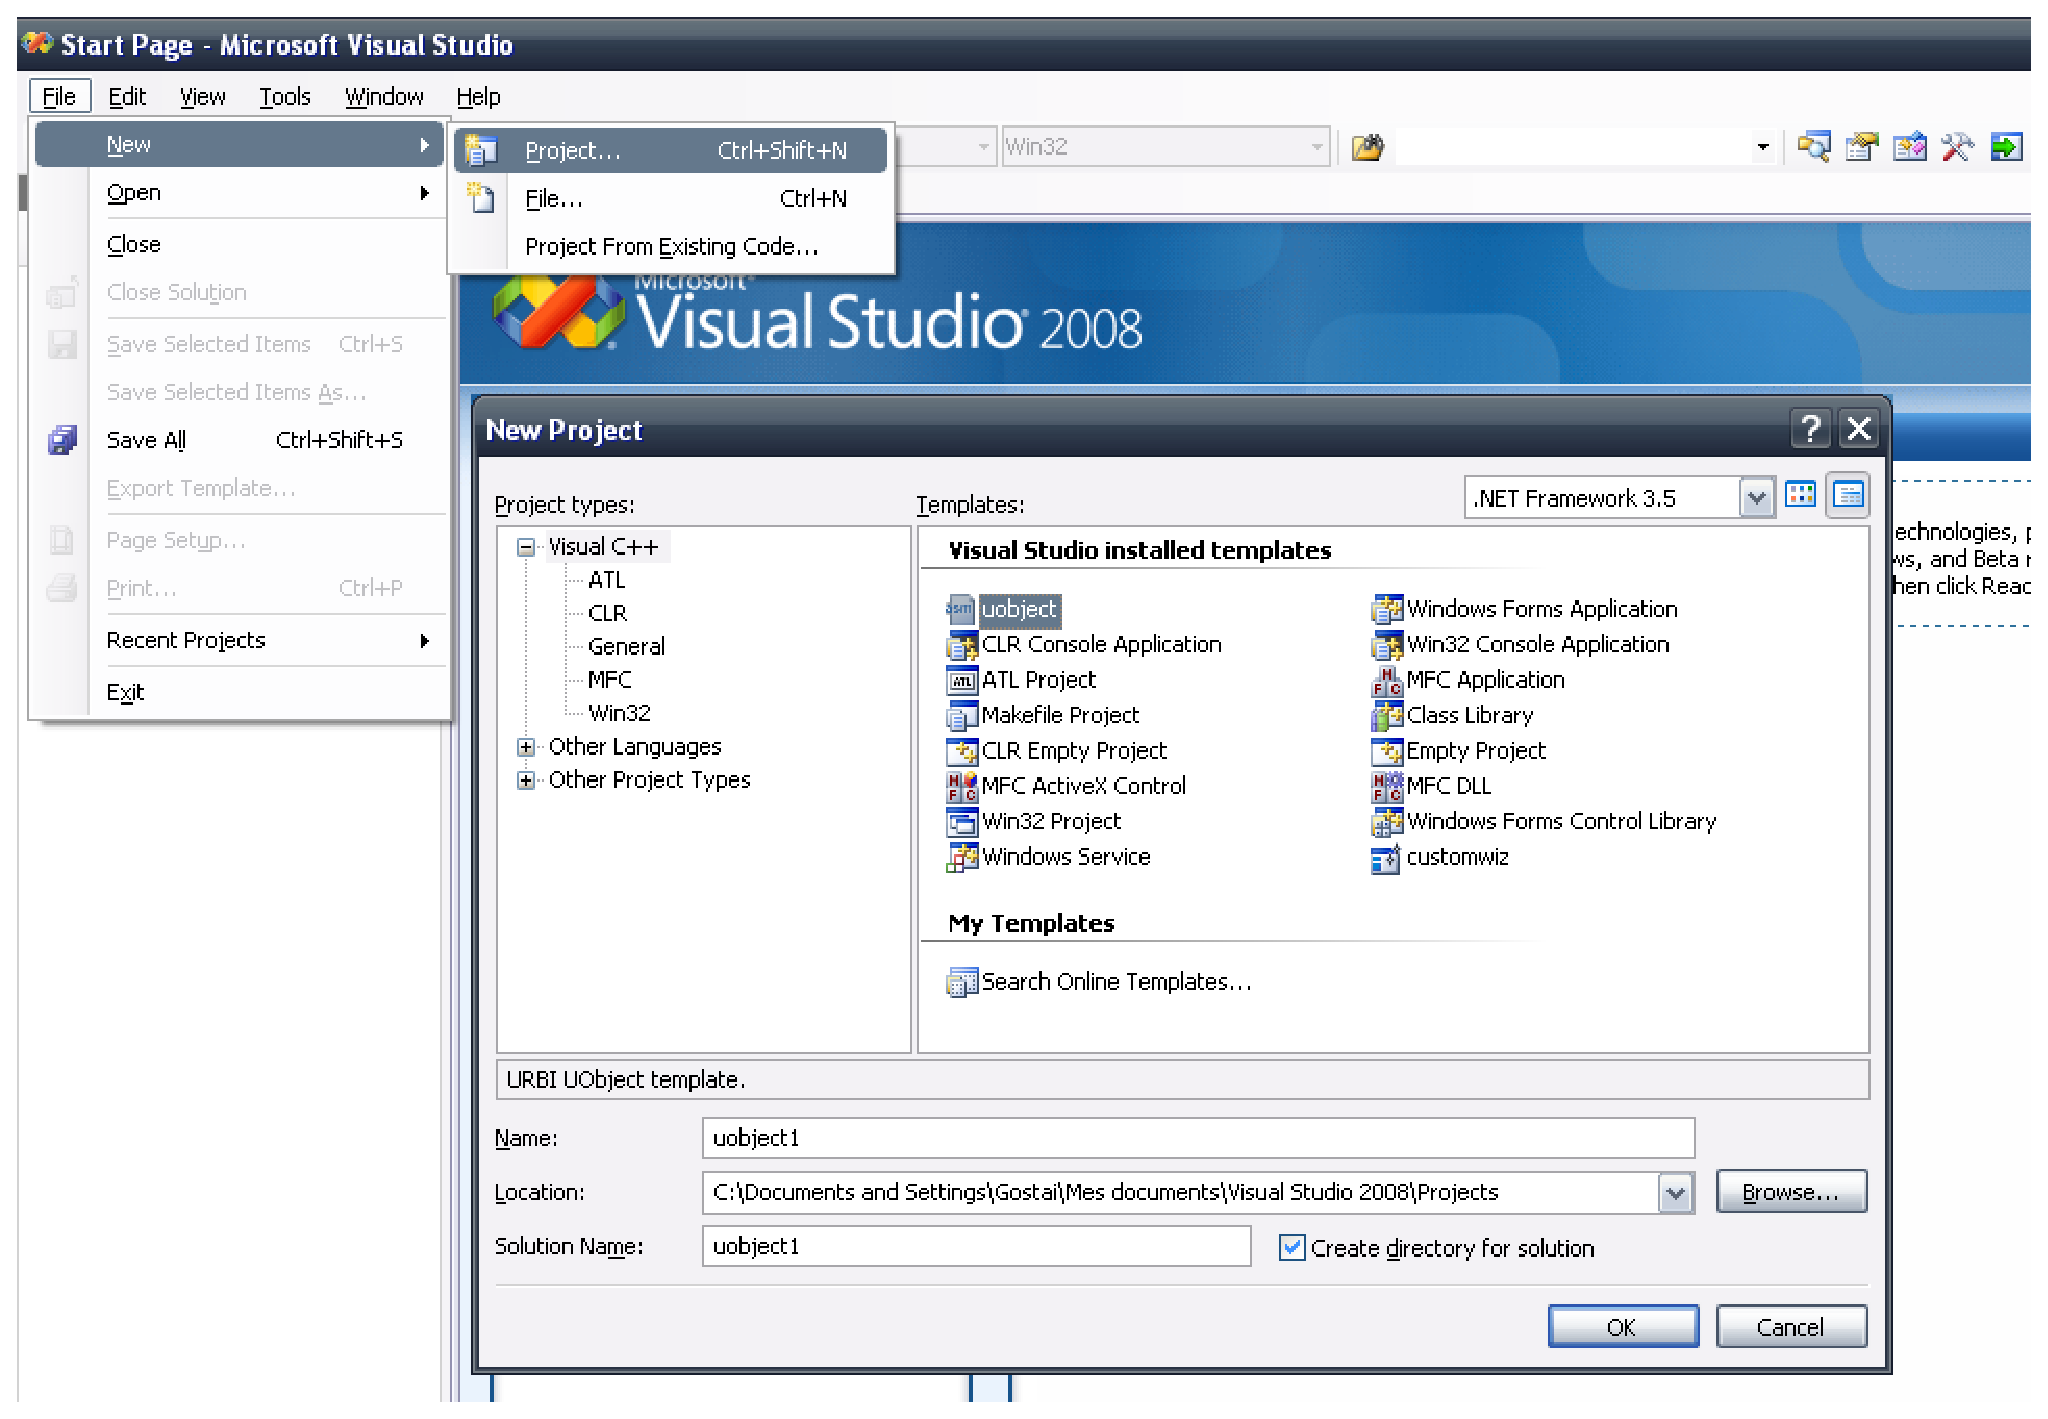
\includegraphics[width=0.6\linewidth]{img/visual-wizard-1}
\end{center}

Then, compile your UObject.

\begin{center}
  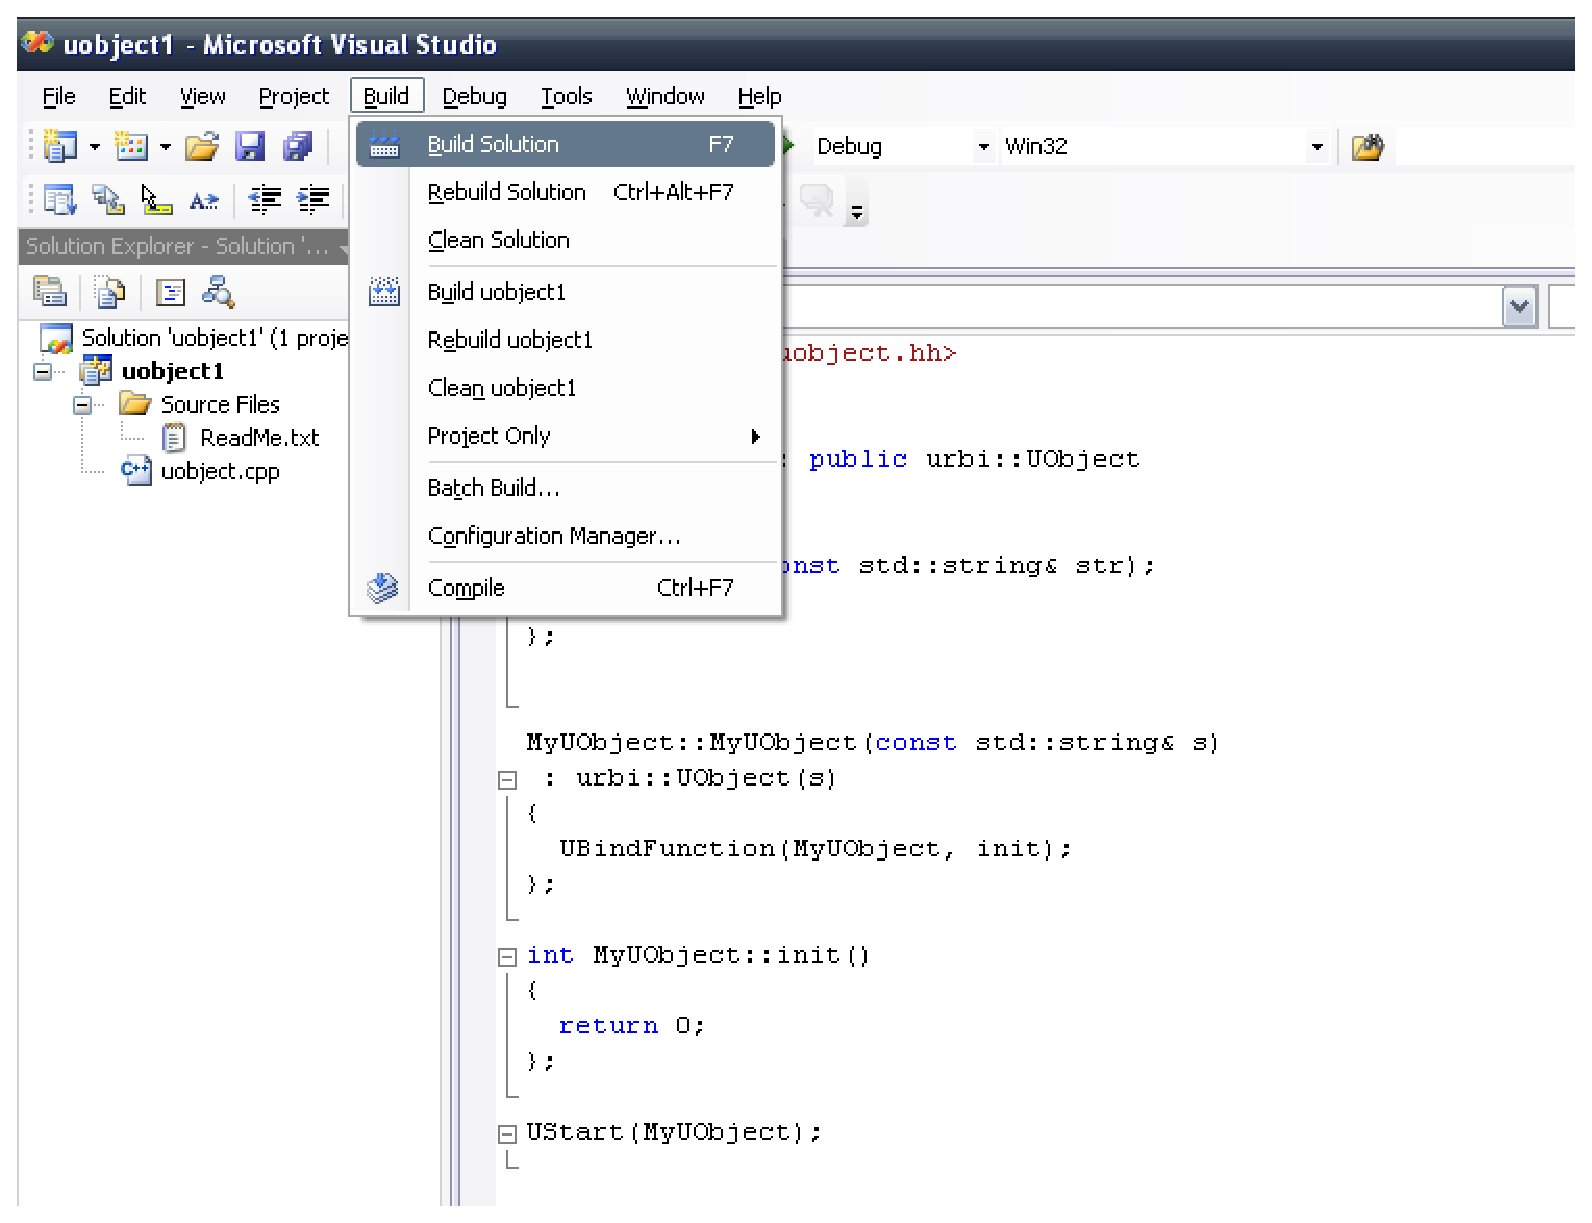
\includegraphics[width=0.6\linewidth]{img/visual-wizard-2}
\end{center}

And run it.

\begin{center}
  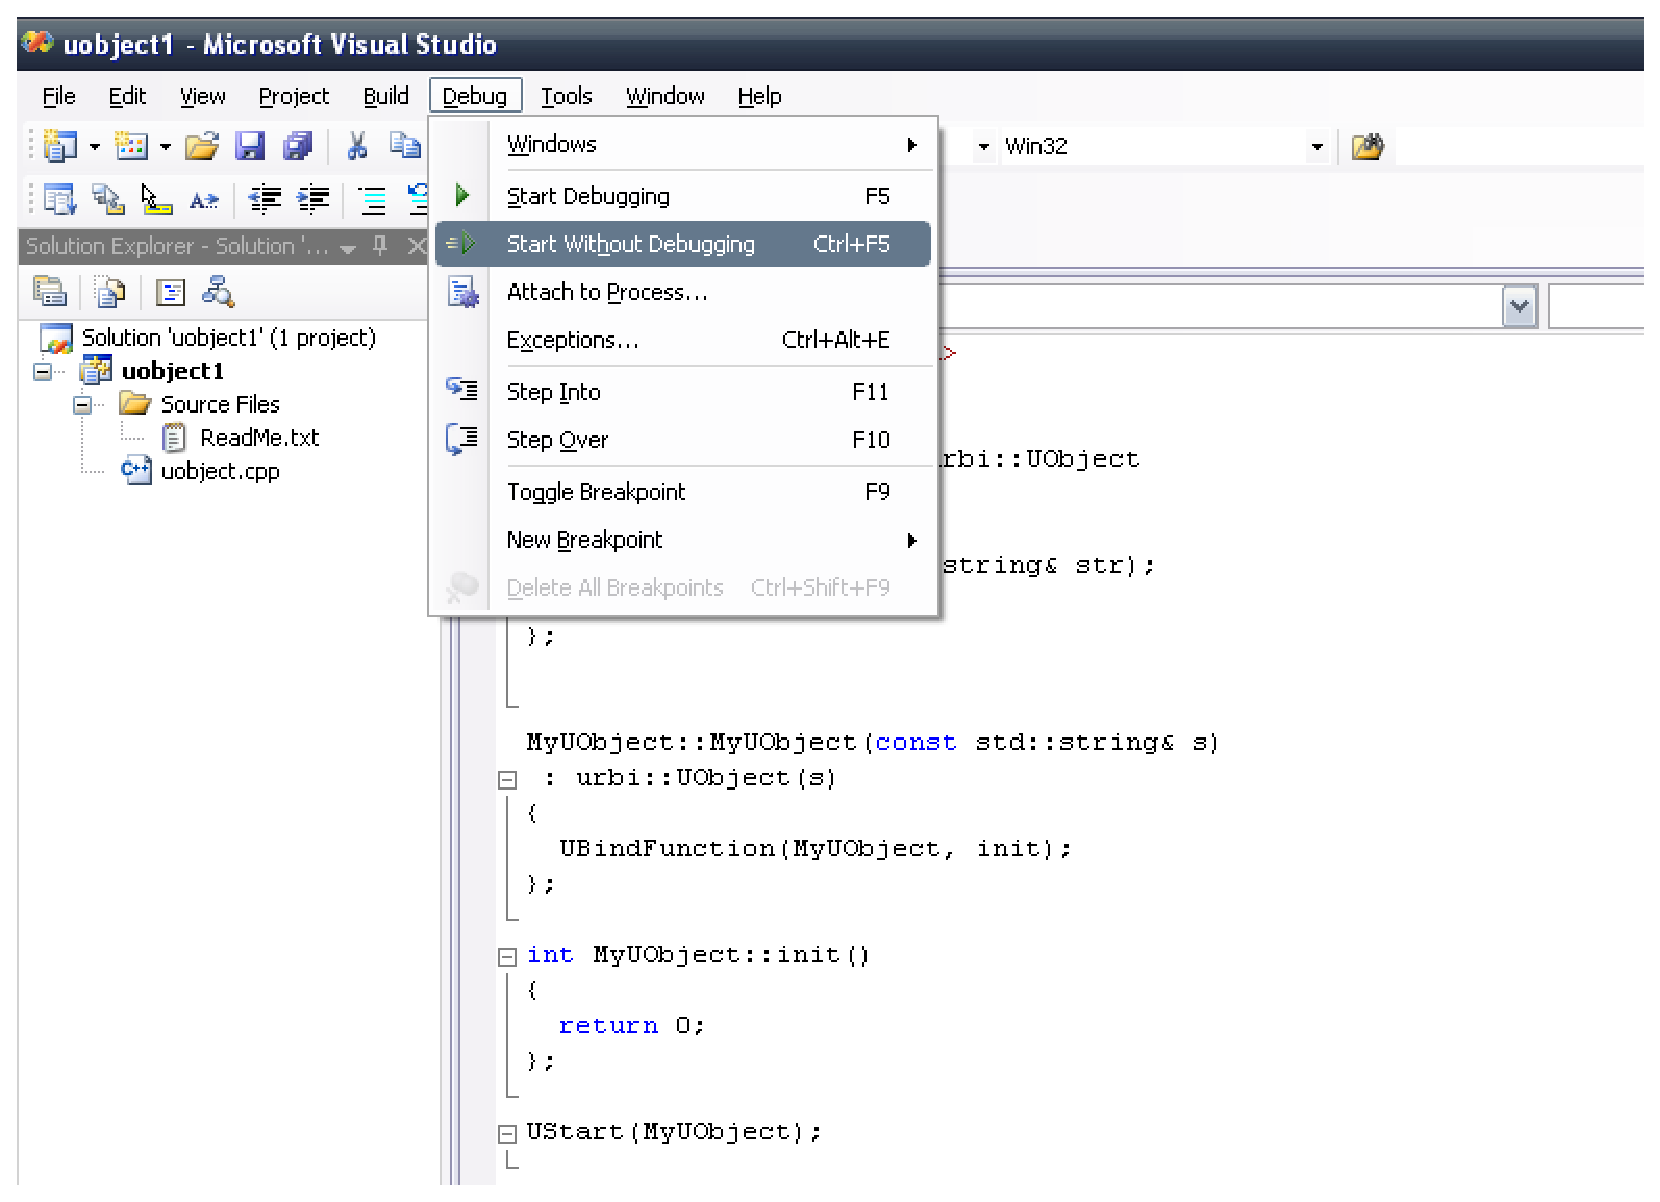
\includegraphics[width=0.6\linewidth]{img/visual-wizard-3}
\end{center}


\section{Creating a class, binding variables and functions}
\label{sec:uob:api:bind}

Let's illustrate those concepts by defining a simple object:
\lstinline{adder}. This object has one variable \lstinline{v}, and a
method \lstinline{add} that returns the sum of this variable and its
argument.

\begin{itemize}
\item First the required include:

\begin{cxx}
#include <urbi/uobject.hh>
\end{cxx}

\item Then we declare our \lstinline{adder} class:
\begin{cxx}
class adder : public urbi::UObject // Must inherit from UObject.
{
  public:
   // The class must have a single constructor taking a string.
   adder (const std::string&);

   // Our variable.
   urbi::UVar v;

   // Our method.
   double add (double);
};
\end{cxx}
\item The implementation of the constructor and our \lstinline{add}
  method:
\begin{cxx}
// the constructor defines what is available from Urbi
adder::adder (const std::string& s)
  : UObject (s) // required
{
  // Bind the variable.
  UBindVar (adder, v);

  // Bind the function.
  UBindFunction (adder, add);
}

double
adder::add (double rhs)
{
  return v + rhs;
}
\end{cxx}
\item And register this class:
\begin{cxx}
// Register the class to the Urbi kernel.
UStart (adder);
\end{cxx}
\end{itemize}

To summarize:

\begin{itemize}
\item Declare your object class as inheriting from
  \lstinline{urbi::UObject}.
\item Declare a single constructor taking a string, and pass this
  string to the constructor of \lstinline{urbi::UObject}.
\item Declare the variables you want to share with \urbi with the type
  \lstinline{urbi::UVar}.
\item In the constructor, use the macros
  \lstinline|UBindVar(\var{class-name}, \var{variable-name})|
  for each \UVar you want as an instance variable, and
  \lstinline|UBindFunction(\var{class-name}, \var{function-name})| for
  each function you want to bind.
\item Call the macro \lstinline{UStart} for each object.
\end{itemize}

\section{Creating new instances}

When you start an \urbi server, an object of each class registered
with \lstinline{UStart} is created with the same name as the
class. New instances can be created from \urbi using the
\lstinline|new| method. For each instance created in \urbi, a
corresponding instance of the \Cxx object is created. You can get the
arguments passed to the constructor by defining and binding a method
named \lstinline|init| with the appropriate number of arguments.

\section{Binding functions}

\subsection{Simple binding}

You can register any member function of your \UObject using the macro

% Fix line wrap.
\lstinline|UBindFunction(\var{class-name}, \var{function-name})|.

Once done, the function can be called from \us.

The following types for arguments and return value are supported:

\begin{itemize}
\item Basic integer and floating types (int, double, float...).
\item \lstinline{const std::string&} or \lstinline{const char*}.
\item \lstinline{urbi::UValue} or any of its subtypes (\UBinary, \UList...).
\item \lstinline{std::list} or \lstinline{std::vector} of the above types.
\end{itemize}

\subsection{Asynchronous binding}
Functions bound using \lstinline{UBindFunction} are called synchronously, and
thus block everything until they return.

If you wish to bind a function that requires a non-negligible amount of time
to execute, you can have it execute in a separate thread by calling

% Separate line since lstinline does not word-wrap and this one is quite long.
\lstinline|UBindThreadedFunction(\var{class-name}, \var{function-name}, \var{lockMode})|.

The function code will be executed in a separate thread without breaking the
\us execution semantics.

The \lstinline{lockMode} argument can be used to prevent parallel execution
of multiple bound functions if your code is not thread-safe. It can be any of
\lstinline{LOCK_NONE}, \lstinline{LOCK_FUNCTION}, \lstinline{LOCK_INSTANCE},
\lstinline{LOCK_CLASS} or \lstinline{LOCK_MODULE}.
When set to \lstinline{LOCK_NONE}, no locking is performed. Otherwise, it
limits parallel executions to:

\begin{itemize}
\item One instance of the bound function for \lstinline{LOCK_FUNCTION}.
\item One bound function for each object instance for
\lstinline{LOCK_INSTANCE}.
\item One bound function for the class for \lstinline{LOCK_CLASS}.
\item One bound function for the whole module (shared object) for
\lstinline{LOCK_MODULE}.
\end{itemize}

There is however a restriction: you cannot mix multiple locking modes: for
instance a function bound with \lstinline{LOCK_FUNCTION} mode will not prevent
another function bound with \lstinline{LOCK_INSTANCE} from executing in
parallel.

You can perform your own locking using semaphores if your code needs a more
complex locking model.

You can limit the maximum number of threads that can run in parallel by using
the \lstinline{setThreadLimit} function.

\section{Notification of a variable change or access}
\label{sec:uobject:uvar-notify}
You can register a function that will be called each time a variable
is modified or accessed (for embedded components only) by calling
\lstinline{UNotifyChange} and \lstinline{UNotifyAccess}, passing
either an \UVar or a variable name as first argument, and a member
function of your \UObject as second argument. This function can take
zero or one argument: a \UVar reference pointing to the \UVar being
accessed or modified. The \lstinline{notifyChange} callback function
is called after the variable value is changed, whereas the
\lstinline{notifyAccess} callback is called before the variable is
accessed, giving you the possibility to update its value.

The callback functions are expected to return a value of type
\lstinline|UReturn|, currently typedefed as an int. This return value
is ignored in the current implementation.

Notify functions can be unregistered by calling the
\lstinline|unnotify| function of the \UVar class.

\section{Data-flow based programming: exchanging UVars}

The \lstinline{UNotifyChange} and \lstinline{UNotifyAccess} features
can be used to link multiple UObjects together, and perform data-flow
based programming: the \lstinline{UNotifyChange} can be called to
monitor UVars from other UObjects.  Those UVars can be transmitted
through bound function calls.

One possible pattern is to have each data-processing UObject take its
input from monitored UVars, given in its constructor, and output the
result of its processing in other UVars. Consider the following
example of an object-tracker:

\begin{cxx}
class ObjectTracker: public urbi::UObject
{
  ObjectTracker(const std::string& n)
    : urbi::UObject(n)
  {
    // Bind our constructor.
    UBindFunction(ObjectTracker, init);
  }
  // Take our data source in our constructor.
  int init(UVar& image)
  {
    UNotifyChange(image, &ObjectTracker::onImage);
    // Bind our output variable.
    UBindVar(ObjectTracker, val);
    return 0;
  }
  int onImage(UVar& src)
  {
    UBinary b = src;
    // Processing here.
    val = processing_result;
    return 0;
  }
  UVar val;
};
UStart(ObjectTracker);
\end{cxx}

The following \us code would be used to initialize an ObjectTracker given a
camera:

\begin{urbiunchecked}
var tracker = ObjectTracker.new(camera.getSlot("val"));
\end{urbiunchecked}

An other component could then take the tracker output as its input.

Using this model, chains of processing elements can be created. Each time the
UObject at the start of the chain updates, all the notifyChange will be called
synchronously in cascade to update the state of the intermediate components.

\section{Timers}
\label{sec:uob:timers}

The API provides two methods to have a function called periodically:
\begin{cxxapi}
\item[void urbi::UObject::USetUpdate(ufloat period)]
  Set up a timer that calls the virtual method
  \lstinline{UObject::update()} with the specified period (in
  milliseconds).  Disable updates if \var{period} is -1.

\item[urbi::TimerHandle urbi::UObject::USetTimer<T>(ufloat period, int (T::*fun)())]
  Invoke an UObject member function \var{fun} every \var{period}
  milliseconds.  \var{fun} is a regular member-function pointer, for
  instance \lstinline|MyUObject::my_function|.
  The function returns a \lstinline|TimerHandle| that can be passed to the
  \lstinline|UObject::removeTimer(h)| function to disable the timer.
\end{cxxapi}

\section{The special case of sensor/effector variables}

In \urbi, a variable can have a different meaning depending on whether
you are reading or writing it: you can use the same variable to
represent the target value of an effector and the current value
measured by an associated sensor. This special mode is activated by
the \UObject defining the variable by calling
\lstinline{UOwned} after calling \lstinline{UBindVar}. This call has
the following effects:
\begin{itemize}
\item When \urbi code or code in other modules read the variable, they
  read the current value.
\item When \urbi code or code in other modules write the variable,
  they set the target value.
\item When the module that called \lstinline|UOwned| reads the
  variable, it reads the target value. When it writes the variable, it
  writes the current value.
\end{itemize}

\section{Using \urbi variables}

You can read or write any \urbi variable by creating an
\UVar passing the variable name to the constructor. Change
the value by writing any compatible type to the \UVar, and
access the value by casting the \UVar to any compatible
type.

Some care must be taken in remote mode: changes on the
variable coming from \urbi code or an other module can take time to propagate
to the \UVar. To have more control on the bandwidth used, you can
disable the automatic update by calling \lstinline|unnotify()|. Then you can get
the value on demand by calling
\lstinline|UNotifyOnRequest (\var{variable}, \var{function})|. Then to get an
updated value, call the \lstinline{requestValue} method on the
\UVar, and your callback function will be called as soon as
the value is available.

You can read and write all the \urbi properties of an \UVar by
reading and writing the appropriate \lstinline{UProp} object in the
\UVar.

\section{Emitting events}

The \UEvent class can be used to create and emit \us events. Instances are
created and initialized exactly as \UVar: either by using the
\lstinline{UBindEvent} macro, or by calling one of its constructors or the
\lstinline{init} function.

Once initialized, the \lstinline{emit} function will trigger the emission of
the associated \us event. It can be called with any number of arguments, of
any compatible type.

\section{UObject and Threads}

The \UObject API is thread-safe in both plugin and remote mode: All API calls
including operations on \UVar can be performed from any thread.

\section{Using binary types}

\urbi can store binary objects of any type in a generic container, and
provides specific structures for sound and images. The generic
containers is called \UBinary and is defined in the
\file{urbi/ubinary.hh} header. It contains an enum field type
giving the type of the binary (\lstinline{UNKNOWN}, \lstinline{SOUND}
or \lstinline{IMAGE}), and an union of a \USound and
\UImage struct containing a pointer to the data, the size
of the data and type-specific meta-information.

\subsection{UVar conversion and memory management}
The \UBinary manages its memory: when destroyed (or going out-of-scope), it
frees all its allocated data. The \USound and \UImage do not.

Reading an \UBinary from a \UVar, and writing a
\UBinary, \USound or \UImage to an \UVar performs a deep-copy of the
data (by default, see below).

Reading a \USound or \UImage from an \UVar performs a shallow copy. Modifying
the data is not allowed in that case.

\subsection{0-copy mode}
In plugin mode, you can setup any \UVar in 0-copy mode by calling
\lstinline{setBypass(true)}. In this mode, binary data written to the \UVar
is not copied, but a reference is kept.
As a consequence, the data is only available from within registered
notifyChange callbacks. Those callbacks can use \lstinline|UVar::val()| or
cast the \UVar to a \UBinary\& to retrieve the reference.
Attempts to read the \UVar from outside notifyChange will result in
\lstinline{nil} being returned.

\section{Using hubs to group objects}

Sometimes, you need to perform actions for a group of
\lstinline{UObjects}, for instance devices that need to be updated
together. The API provides the \UObjectHub class for this
purpose. To create a hub, simply declare a subclass of
\UObjectHub, and register it by calling once the macro
\lstinline|UStartHub (\var{class-name})|. A single instance of this class
will then be created upon server start-up. \UObject
instances can then register to this hub by calling
\lstinline|URegister (\var{hub-class-name})|. Timers can be attached to
\UObjectHub the same way as to \UObject (see
\autoref{sec:uob:timers}). The kernel will call the \lstinline{update()}
method of all \UObject before calling the
\lstinline{update()} method of the hub. A hub instance can be
retrieved by calling \lstinline{getUObjectHub (string classname)}. The
hub also holds the list of registered UObject in its members
attribute.

\section{Sending \urbi code}

If you need to send \urbi code to the server, the \lstinline{URBI()}
macro is available, as well as the \lstinline{send()} function. You
can either pass it a string, or directly \urbi code inside a double
pair of parentheses:

\begin{urbiunchecked}
send ("myTag:1+1;");

URBI (( at (myEvent?(var x)) { myTag:echo x; }; ));
\end{urbiunchecked}

You can also use the \lstinline{call} method to make an urbiscript function
call:

\begin{urbiunchecked}
// C++ equivalent of urbiscript 'System.someFunc(12, "foo");'
call("System", "someFunc", 12, "foo");
\end{urbiunchecked}


%%% Local Variables:
%%% mode: latex
%%% TeX-master: "../urbi-sdk"
%%% ispell-dictionary: "american"
%%% ispell-personal-dictionary: "../urbi.dict"
%%% fill-column: 76
%%% End:
